Wenn eine Applikation entwickelt werden soll, ist die Wahl der richtigen Methode, Frameworks oder auch der Programmiersprache eine wichtige Entscheidung für das Projekt. Viele Entscheidungen können im Verlauf der Entwicklung noch abgeändert werden, aber um eine derartige Entscheidung zu ändern, müssen Teile der Anwendung oder auch der komplette Quellcode neu geschrieben werden. Neben Unsicherheiten bei der richtigen Wahl kommen täglich neue Artikel, warum die eine neue Programmiersprache der neue Standard wird. So ist eine derartig wichtige Entscheidung oft sehr schwierig.

Da Anwendungen meistens nicht nur auf einem Gerätetyp, sondern allen Nutzern auf den verschiedensten Plattformen zur Verfügung stehen sollen, hat diese Entscheidung noch einmal eine größere Bedeutung, da sie eng verbunden mit den Kosten der Entwicklung und dem Nutzungserlebnis ist.

In Zeiten der Heimcomputer und des stetig wachsenden Internets war der einfachste Weg , eine Webseite zu entwickeln, die über den Browser der genutzten Geräte aufgerufen werden konnte. Mit der Ära der Smartphones jedoch änderte sich das. So waren Webapplikationen oft nicht für die Nutzung an derartig kleinen Geräten mit einer Toucheingabe angepasst.

Die Nutzung von Smartphones öffnete außerdem die Tür, andere Funktionalitäten wie die Kamera, Bluetooth oder GPS-Daten zu nutzen. Deshalb wurden Applikationen oft nativ mit Objectiv-C, beziehungsweise Swift, für iOS und Java, mittlerweile Kotlin, für Android entwickelt. Durch die Programmierung mit Hilfe der nativen Programmiersprachen, entstehen optimal für die einzelnen Plattformen angepasste Anwendungen.

Durch den Wunsch nach einer Multi-Plattform Anwendung jedoch, also einer App, die für mehrere Plattformen veröffentlicht werden soll, muss bei der nativen Entwicklung für jede Plattform eine eigene Applikationen in der jeweiligen Programmiersprache und Technologie geschrieben werden. Dadurch entsteht ein sehr hoher Aufwand und die Kosten multiplizieren sich mit der Zahl der abzudeckenden Plattform.

Deswegen wurde bereits früh mit der Entwicklung von sogenannten Cross-Plattform Technologien gestartet, die es ermöglichen sollen, mit einem geteilten Code so viele Plattformen wie möglich abzudecken. So erschien etwa 2008 PhoneGap. Es war ein Open-Source Framework zur Entwicklung von hybriden mobilen Applikationen, die mit Hilfe von HTML, CSS und Javascript programmiert wurden. PhoneGap und sein Nachfolger Cordova waren einige Zeit auch sehr beliebt in diesem Bereich. 2019 hatten beide zusammen immerhin einen Marktanteil von knapp 40\% unter den Cross-Plattform Frameworks \cite{statist_CP_Framework}.

Trotz der veringerten Kosten, werden dennoch viele Applikationen immer noch nativ entwickelt. So ergab eine interne Untersuchung der Firma \verb|ScanBot SDK|\footnote{https://scanbot.io/de/blog/native-apps-vs-cross-platform/}, dass 2019, 57\% ihrer Nutzer native Applikationen entwickelten, obwohl ihr Produkt ebenso für viele der gängigen Cross-Plattform Frameworks zur Verfügung steht.

Ein Grund für Unsicherheit in diesem Bereich sind oft auch negative Erfahrungsberichte von Firmen, die einen Umstieg von nativ zu Cross-Plattform-Applikationen versuchten.  So etwa auch Airbnb \cite{Airbnb_react_goals}. Sie nutzten das von Facebook mitentwickelte Framework React Native. 2019 hatte dieses Framework einen Marktanteil von 42\% \cite{statist_CP_Framework}. 

Ihre Ziele waren einfach:
\begin{enumerate}
    \item Schnelleres entwickeln.
    \item Die gleiche Codequalität beibehalten.
    \item Nur noch eine Codebasis.
    \item Die Entwicklererfahrung verbessern.
\end{enumerate}
Jedoch traten während der Entwicklung einige technische Probleme auf, die dazu führten, dass sie ihre Ziele nicht einhalten konnten und 2018 wieder zu einem nativen Ansatz zurückkehrten.

Durch Beispiele wie dieses, waren und sind App-Entwickler oft skeptisch gegenüber derartigen Lösungen, da dies auch immer mit großen Änderungen und hohen Investitionen verbunden sind. Dennoch ist der Wille da und auch die Zahl der Cross-Plattform Entwicklungen nimmt in den letzten Jahren zu. So ergab die Untersuchung von \verb|ScanBot SDK|, dass 2021, gerade einmal zwei Jahre später 58\% Cross-Plattform Lösungen nutzten, also ganze 15\% mehr. Diese Zahl stützt auch eine Untersuchung von Jetbrains. Diese ergab, dass 2021 53\% aller App Entwickler, derartige Technologien nutzen \cite{JetBrains_miscellaneous_2021}.

\begin{figure}[ht]
  \centering
  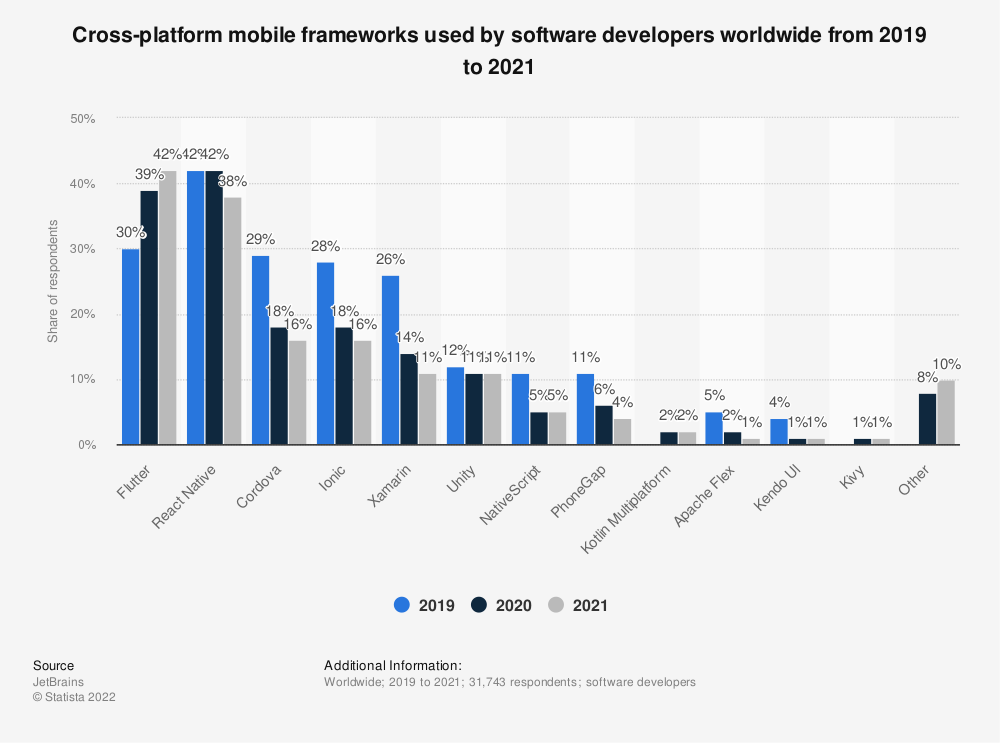
\includegraphics[height=7cm,keepaspectratio]{images/cross-platform-mobile-frameworks.png} 
  \caption[Statistik Cross-Plattform-Frameworks]{Cross-Plattform-Frameworks 2019-2021 \cite{statist_CP_Framework}}
  \label{fig:statista_cross_plattform}
\end{figure}

Diese Zahl dürfte sich auch noch in den nächsten Jahren weiter erhöhen. Einen Grund dafür bietet unter anderem auch die neuen Technologien die entstehen. So etwa Flutter. In Abbildung \ref{fig:statista_cross_plattform} ist eine Statistik zu sehen, die die Verteilung von verschiedenen Cross-Plattform-Entwicklungstechnologien zeigt. Sie zeigt eindrucksvoll wie schnell sich die Verteilung von Cross-Platform Frameworks ändern kann. Flutter ist dafür ein gutes Beispiel. Es ist ein Framework das erst 2017 auf den Markt gekommen ist und innerhalb von gerade einmal 4 Jahren auf einen Marktanteil von 42\% gekommen ist. Von einigen wird es als der neue Standard angesehen und viele Unternehmen steigen auf Flutter um oder bekunden großes Interesse daran. 

Jedoch gibt es auch Entwickler, die wegen Unsicherheiten und einigen anderen Gründen immer noch nativ entwickeln. So entwickelt die Number42 alle ihre betreuten mobilen Applikationen mit den nativen Programmiersprachen. Denn auch die nativen Programmiersprachen entwickeln sich stetig weiter und bekommen Änderungen, die eine Entwicklung vereinfachen und beschleunigen. Dadurch ist auch dieser Ansatz nicht von der Hand zu weisen und es kann durchaus sinnvoll sein, neue Apps weiterhin nativ zu entwickeln.

\section{Einordnung der Arbeit}
Diese Arbeit soll zunächst einen geordneten Überblick über die verschiedenen Entwicklungsansätze geben und somit eine gemeinsame Grundlage bilden, da es viele verschiedene Einordnungen gibt.
Danach soll anhand von verschiedenen Implementierungen eine Untersuchung von vier verschiedenen Ansätzen gemacht werden, um einige der vorgestellten Ansätze genauer zu betrachten.
Am Schluss soll anhand der verschiedenen Implementierungen und Erfahrungen während der Entwicklung ein Vergleich zwischen den ausgewählten Ansätzen gezogen werden und daraus ein Fragekatalog erstellt werden, der die Wahl eines passenden Ansatzes erleichtern soll.


\section{Aufbau der Arbeit}
Diese Arbeit hat 6 Kapitel. Eine Einleitung und Motivation ist in Kapitel 1 zu finden. In Kapitel 2 werden verwandten Arbeiten vorgestellt, während in Kapitel 3 die verschiedenen App-Arten, das Projekt, die verschiedenen Implementierungen vorgestellt und eine Abgrenzung der Arbeit stattfindet.
Danach werden in Kapitel 4 die verschiedenen Implementierungen genauer erklärt und einige Bemerkung zu der Entwicklung getroffen. Dabei soll auch auf Stärken und Schwächen der einzelnen Implementierungen eingegangen werden, die während der Implementierung und Recherche aufgefallen sind.
In Kapitel 5 soll anschließend eine Auswertung der einzelnen Entwicklungsansätze stattfinden und anhand einiger Kriterien und weiterer Erklärungen ein Vergleich gezogen werden. Zusätzlich wird anhand eines Fragenkatalogs mit Begründungen ein Entscheidungskompass vorgestellt, der bei der Auswahl eines Ansatzes helfen soll. Abschließend soll in Kapitel 6 ein Fazit gezogen werden und ein Ausblick auf künftige Arbeiten aufgezeigt werden.